\documentclass[11pt]{article}
\usepackage[utf8]{inputenc}
\usepackage[portuguese, english]{babel}
\usepackage[T1]{fontenc}
\usepackage{subfigure} 
\usepackage{lmodern}
\usepackage{geometry}
\usepackage{authblk}
\usepackage{graphicx}
\usepackage{multicol}
\usepackage{multirow}
\usepackage{float} 
\usepackage{amsmath}

\newcommand\scalemath[2]{\scalebox{#1}{\mbox{\ensuremath{\displaystyle #2}}}}

\geometry{legalpaper, margin=1in}
\renewcommand{\arraystretch}{1.15}

\begin{document}


%%%%%%%%%%%%%%%%%%%%%%%%%%%%%%%%%%%%%%%%%%%%%%%%%%%%%%%%%%%%%%%%%%%%%%%%
%                                                                      %
%     File: Thesis_FrontCover.tex                                      %
%     Tex Master: Thesis.tex                                           %
%                                                                      %
%     Author: Andre C. Marta                                           %
%     Last modified :  2 Jul 2015                                      %
%                                                                      %
%%%%%%%%%%%%%%%%%%%%%%%%%%%%%%%%%%%%%%%%%%%%%%%%%%%%%%%%%%%%%%%%%%%%%%%%

\thispagestyle {empty}

% IST Logo - Signature A
% parameters: bb=llx lly urx ury (bounding box), width=h_length, height=v_length, angle=angle, scale=factor, clip=true/false, draft=true/false. 

\includegraphics[bb=9.5cm 11cm 0cm 0cm,scale=0.29]{IST_A_CMYK_POS}

\begin{center}
%
% Figure (Image or plot)
\vspace{1.0cm}
% height = 50 mm
%\includegraphics[height=50mm]{Figures/Airbus_A350.jpg}

% Title, author and degree
\vspace{1cm}
{\FontLb Circuit Theory and Electronics Fundamentals} \\ % <<<<< EDIT TITLE
\vspace{1cm}
{\FontSn Department of Electrical and Computer Engineering, Técnico, University of Lisbon} \\ % <<<<< EDIT COURSE
\vspace{1cm}
{\FontSn Example Laboratory Report} \\
\vspace{1cm}
{\FontSn February 27, 2021} \\ % <<<<< EDIT DATE (corresponds to date of oral examination)
%
\end{center}


\maketitle

\renewenvironment{abstract}[1]
  {\bigskip\selectlanguage{#1}%
   \begin{center}\bfseries\abstractname\end{center}}
  {\par\bigskip}

\begin{abstract}{english}
    In this report, we show a concise analysis of a 4 single mesh circuit through mesh and nodal analysis. Hitherto Ngspice has been considered a good circuit analyser and thus chosen it was to run the same circuit for comparison with the aforementioned theoretical analysis.
\end{abstract}
\tableofcontents
\addcontentsline{toc}{section}{\listtablename}
\listoftables
\addcontentsline{toc}{section}{\listfigurename}
\listoffigures
\cleardoublepage

\section{Introduction}
The main goal of this laboratory assignment is to design, implement and analyse a band-pass filter (BPF) using an OP-AMP (operational amplifier) having in mind that it should have a good relation efficiency-price. The final objective was to get a central frequency of $1kHz$ for the output signal and a voltage gain of $40dB$ and the circuit's efficiency will be measured considering these objectives that were set. \\

So, in order to evaluate the relation efficiency-price of the built circuit, we will use a merit figure that considers the total cost of the circuit and the deviation to the desired gain and central frequency, defined as:

\begin{equation}
    M = \frac{1}{cost \cdot |40 - gain| \cdot |1000 - central freq.|}
    \label{merit}
\end{equation}

To calculate the total cost associated to this circuit, one considered that it equals the sum of the cost of the resistors, capacitors and transistors which is given by:

\begin{table}[H]
    \centering
    \begin{tabular}{|c|c|}
        \hline
        \textbf{Component} &  \textbf{Price}\\
        \hline
        Resistors & 1 MU $k\Omega^{-1}$ \\ \hline
        Capacitors & 1 MU $\mu F^{-1}$ \\ \hline
        Transistors & 0.1 MU transistor$^{-1}$\\
        \hline
    \end{tabular}
    \caption{Price table for the components used}
    \label{tab:price}
\end{table}

The central frequency represented on eq. \eqref{merit} can be directly calculated from the definition of transfer function for this system and it is given by the geometric mean of the lower and higher cutoff frequencies:

\begin{equation}
    central freq. = \sqrt{f_H f_L}
\end{equation}

in which $f_H$ corresponds to the higher cutoff frequency and $f_L$ to the lower cutoff frequency. Finally, the value for the voltage gain used on eq. \eqref{merit} is easily obtained as the correspondent voltage value for the central frequency obtained. \\

The circuit used to implement this band-pass filter using an OP-AMP can be divided in 3 main regions as it can be seen on Fig. \ref{initialscheme}

\begin{figure}[H]
    \centering
    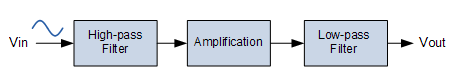
\includegraphics{esquemabunituh.PNG}
    \caption{Simplified scheme to present the 3 regions in which the circuit used can be divided}
    \label{initialscheme}
\end{figure}

The first part, a high-pass filter stage, will essentially have a resistor and a capacitor (i.e. will only pass signals with a frequency higher than a certain cutoff frequency, $f_L$). This part is followed by an amplification unit which will have the main objective of increasing the output voltage gain and which counts with an OP-AMP and two resistors. Finally, one implemented a low-pass filter stage on the circuit which operates on the opposite way of the high-pass filter, i.e. blocks all the signals with a frequency higher than a certain cutoff frequency, $f_H$). \\

As it is trivial, the high-pass filter and the low-pass filter blocking simultaneously frequencies lower than $f_L$ and higher that $f_H$ will act as a band-pass filter as desired. \\

Furthermore, and considering all the points mentioned before, the circuit used for this purpose was the following:


The results were obtained through a theoretical analysis, in which one predicted the output by using a theoretical method that suited the real circuit and through a simulation that was made using \textit{Ngspice}. The results obtained through both methods will be analysed throughout the report. However, because the models used in \textit{Ngspice} are more correct than the ones used on the theoretical analysis, any type of optimization was done almost exclusively in the simulation analysis.\\
\section{Simulation Analysis and the Path for the Greater Good}

For this analysis, we used the default diode model available in \textit{Ngspice}, having then created the circuit presented in Fig. \ref{fig:bigscheme} (it was using Ngspice that we determined, in fact, what was the best circuit for our purposes). So, we used the following chain of thought in order to do what we did. In the envelope detector part, we took the limit as $R \rightarrow \infty$, which is the same as no current passing through there, which is the same as nothing being there. This drastically reduces our ripples, for then we do not need the resistance at all and the cost is 0. Of course this is slightly counterbalanced by the presence of the $10^{-6}$, in the merit calculation (\eqref{score}).  Knowing that the voltage ripples reduce to \eqref{eq:ripples}
\begin{equation}
    V_{ripple} = v_o(0) - v_o(T) = A \left(1 - e^{-\frac{T}{2RC}}\right)
    \label{eq:ripples}
\end{equation}
we can model very superficially the function that should describe this merit in terms of our components (\eqref{eq:approx}).

\begin{equation}
    f(R,C) = \frac{1}{(R+C)*A*\left(1 - e^{-\frac{T}{2RC}}+ 10^{-6}\right )}
    \label{eq:approx}
\end{equation}

From that, we can then plot what's the aspect of the function, shown in Fig. \ref{fig:plot}.

\begin{figure}[H]
    \centering
    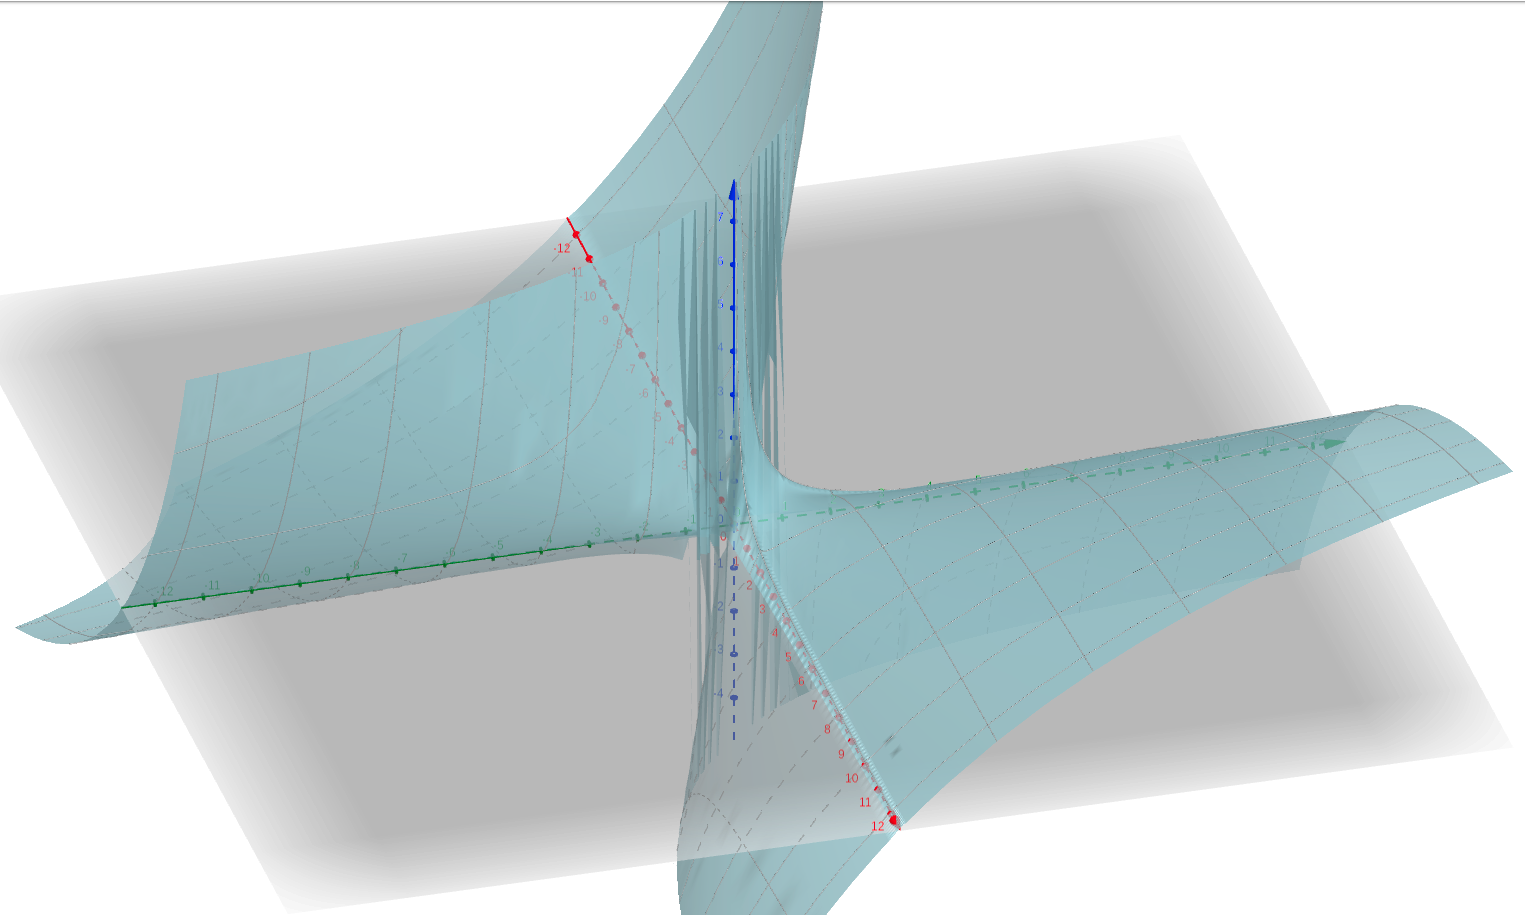
\includegraphics[width = 0.85\linewidth]{cost.png}
        \caption{\textit{Merit approximated function. Plot obtained using GeoGebra3D}}
    \label{fig:plot}
\end{figure}

And thus we have the justification of our doings by removing the resistor. Then, we made use of the specifications of the non-linear part of the diodes and found that there is a very fortunate correlation between the amount of diodes in the voltage regulator and the ripples in the end voltage. What this means is that we can let go of the equation that says that $R2$ must be much greater than $rd$, for this is but a very rough approximation of the real life's diode behaviour. The only setback of this method is the stabilization time, but the merit does not take that into account, so we're good. This way, we used 31 diodes, for nonetheless we did not want to have an exaggerated stabilization time. WARNING: This will cause big differences between the theoretical analysis and the simulation. The model presented in class, when applied to Octave, will basically serve of nothing.

Finally, one found the values considered as the best to find an optimal merit score which are given by:

\begin{table}[H]
    \centering
    \begin{tabular}{|c|c|c|c|}
    \hline
        \textbf{Component} &  \textbf{Amount} & \textbf{Value} & \textbf{Cost}\\
        \hline
        \hline
        Resistors & 1 & $0.2k\Omega$ & 0.2\\
        \hline
        Capacitors & 1 &  $1.33\mu$F & 1.33\\
        \hline
        Diodes & 31+4 & - & 3.5 \\
        \hline
    \end{tabular}
    \caption{Components values shown in Fig. \ref{fig:bigscheme}.}
    \label{tab:tentativas}
\end{table}


\subsection{Cost and Merit Score}
Evaluating the merit, and knowing that the cost is given by \eqref{eq:cost}
\begin{equation}
    c = cost = 35 \cdot 0.1 + 0.2 + 1.33 =  4.85\text{MU}
    \label{eq:cost}
\end{equation}

Using the values obtained for $c$, $d$ and $r$, one can finally calculate the merit score obtained with this circuit (calculated using equation \eqref{score}), which allows one to get the following score:

\begin{equation}
    M = 3.31752e+02
\end{equation}

\subsection{Envelope Detector and Voltage Regulator output voltages}
To understand the role played by the envelope detector and the voltage regulator circuits in our circuit one plotted the results obtained for the output voltages in each one of them. So, starting by the plot obtained at the output terminals of the envelope detector circuit

\begin{equation}
    V = v_4
\end{equation}

Plotting this function:

\vspace{-140px}
\begin{figure}[H]
    \centering
    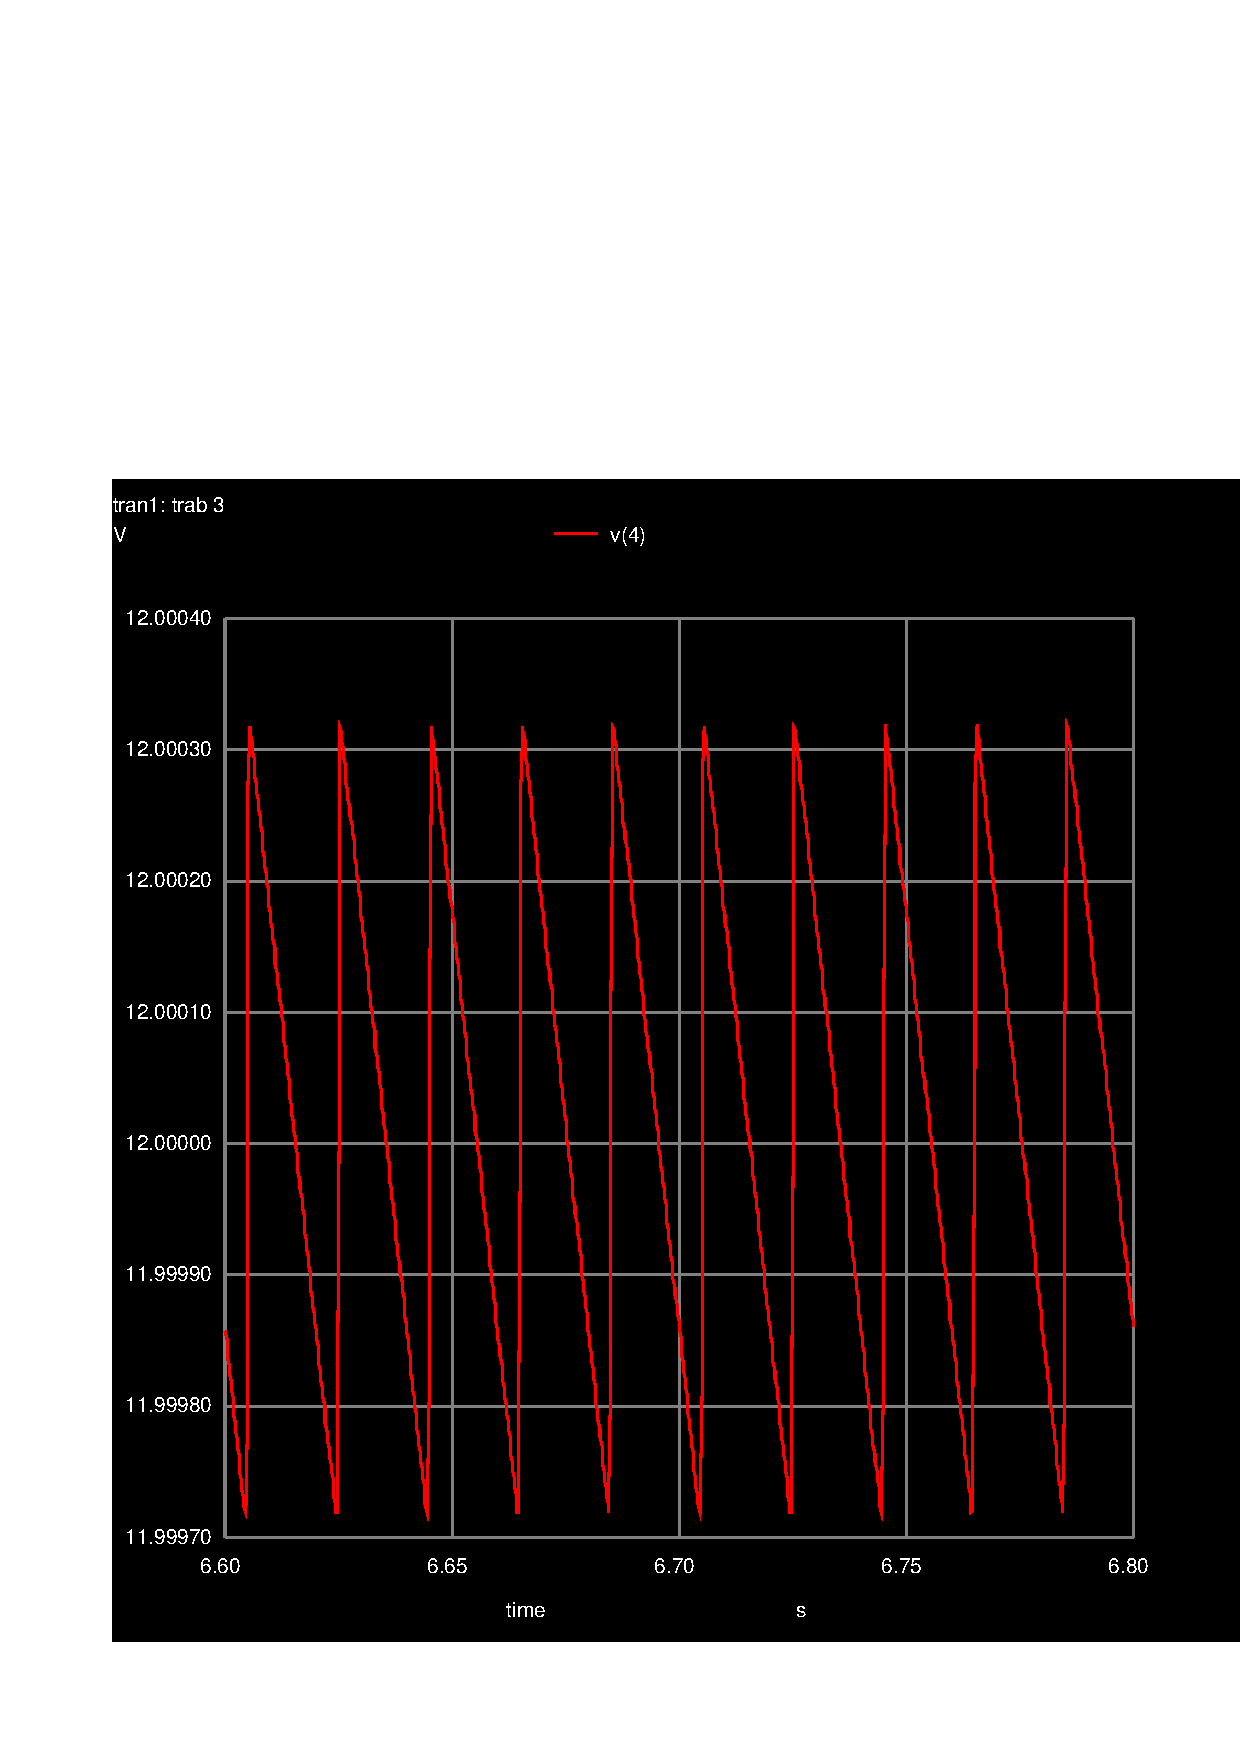
\includegraphics[width = 0.85\linewidth]{sim/antes.pdf}
    \vspace*{-10mm}
        \caption{\textit{Plot of the output voltage registered at the output terminals of the envelope detector circuit}}
    \label{fig:before}
\end{figure}

To plot the output voltage observed on the terminals of the voltage regulator circuit, one plotted the function given by

\begin{equation}
    V = v_5
\end{equation}

which allowed to get

\vspace{-140px}
\begin{figure}[H]
    \centering
    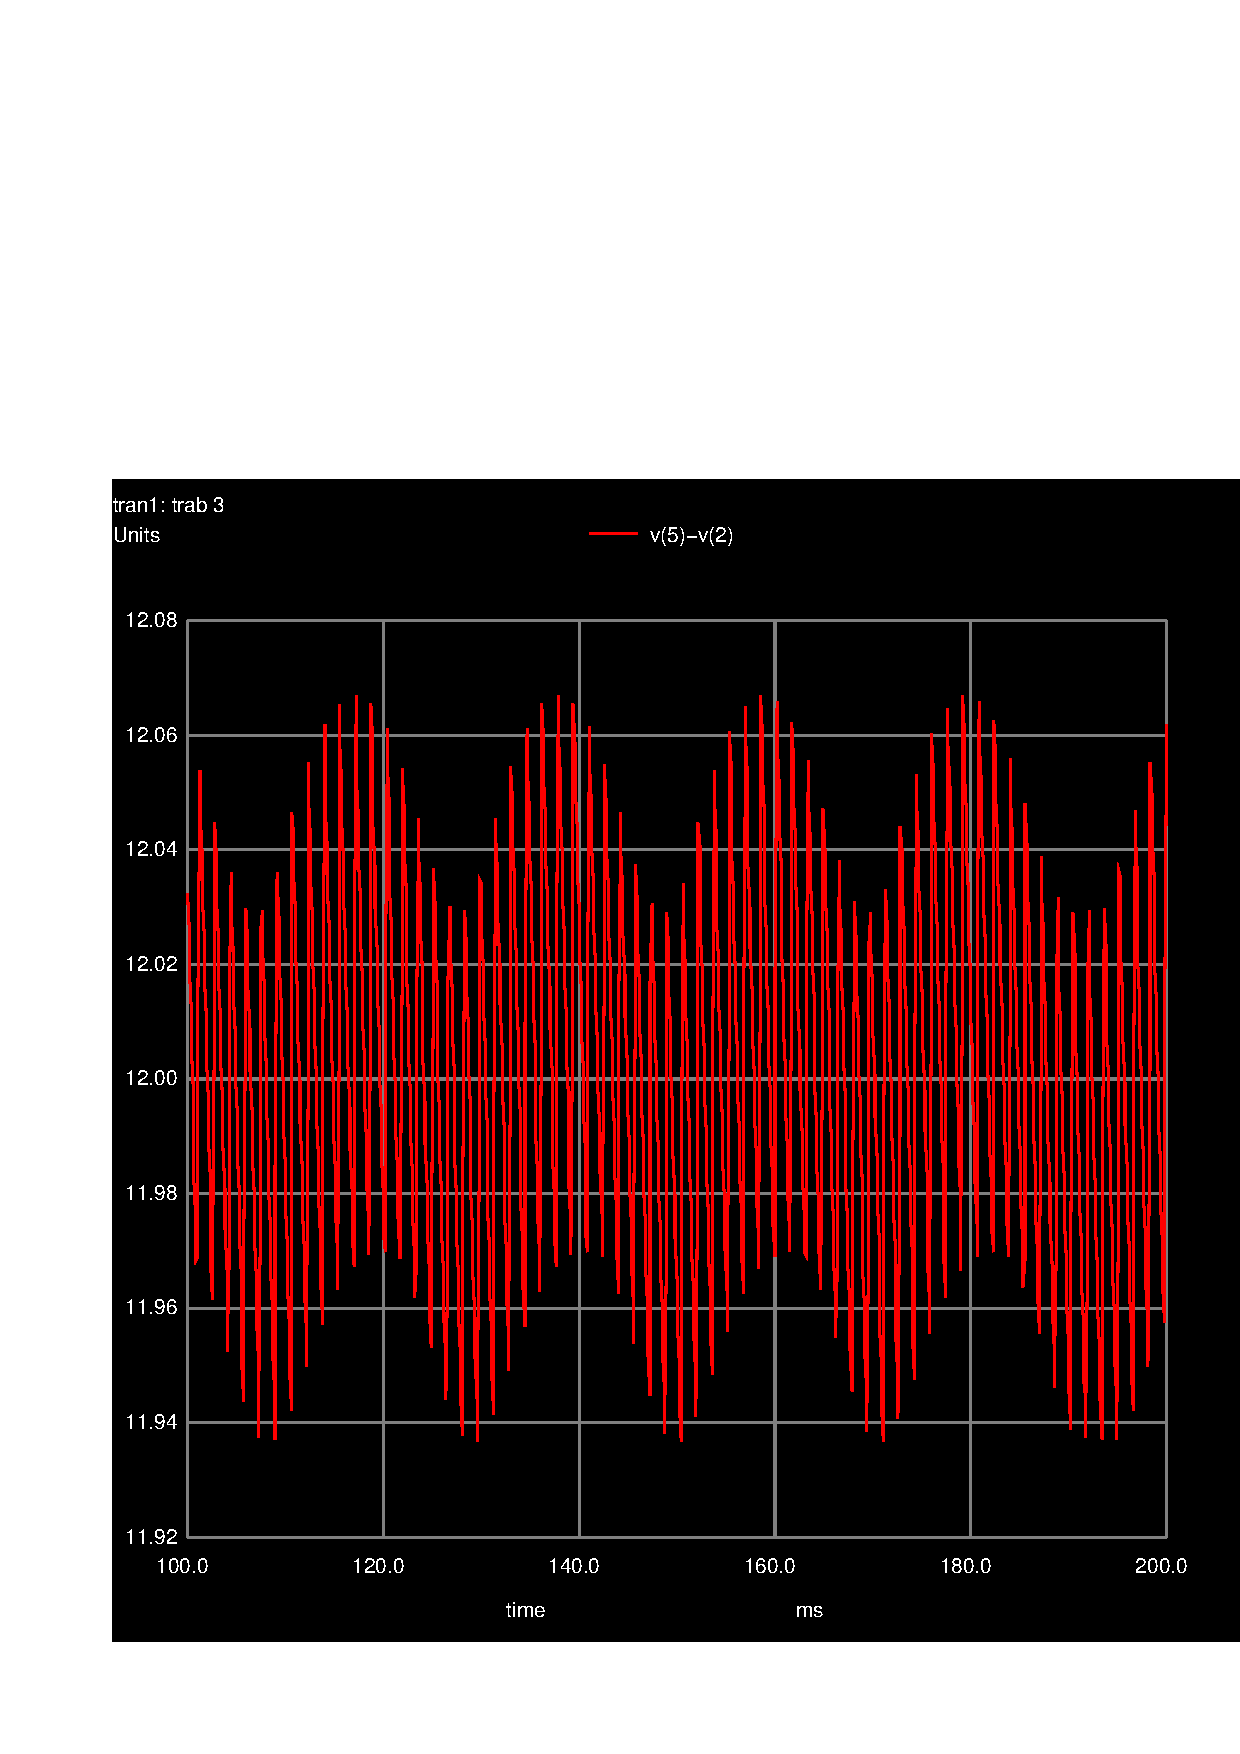
\includegraphics[width = 0.85\linewidth]{sim/zauzau.pdf}
    \vspace*{-10mm}
        \caption{\textit{Plot of the output voltage registered at the output terminals of the voltage regulator circuit}}
    \label{fig:zauzau}
\end{figure}

Comparing the two plots one can conclude that the plots are perfectly similar except on the $y$ axis scale. In fact, the difference between the two plots was caused by the action of our voltage regulator circuit. As the number of diodes was chosen to set an upper limit to the output voltage of the circuit to the desired value $V = 12V$ the difference registered between the two graphs only reflects the effect of that part of the circuit. And in fact, as one can see, the voltage regulator circuit is working as it is supposed to because the voltage that was intially oscillating around $14V$ is oscillating around $12V$ at the output terminals of the voltage regulator. This translates, numerically, into: INSERT HERE
\begin{equation}
    v_{6 average} = 
\end{equation}

\subsection{Plotting $v_o - 12$}
Finally, to conclude the simulation analysis (which one can antecipate that allowed to get precise and satisfactory results) and to better understand how the output voltage behaved next to the desired value of $V = 12V$, one plotted the function $V = v_o - 12$:

\vspace{-140px}
\begin{figure}[H]
    \centering
    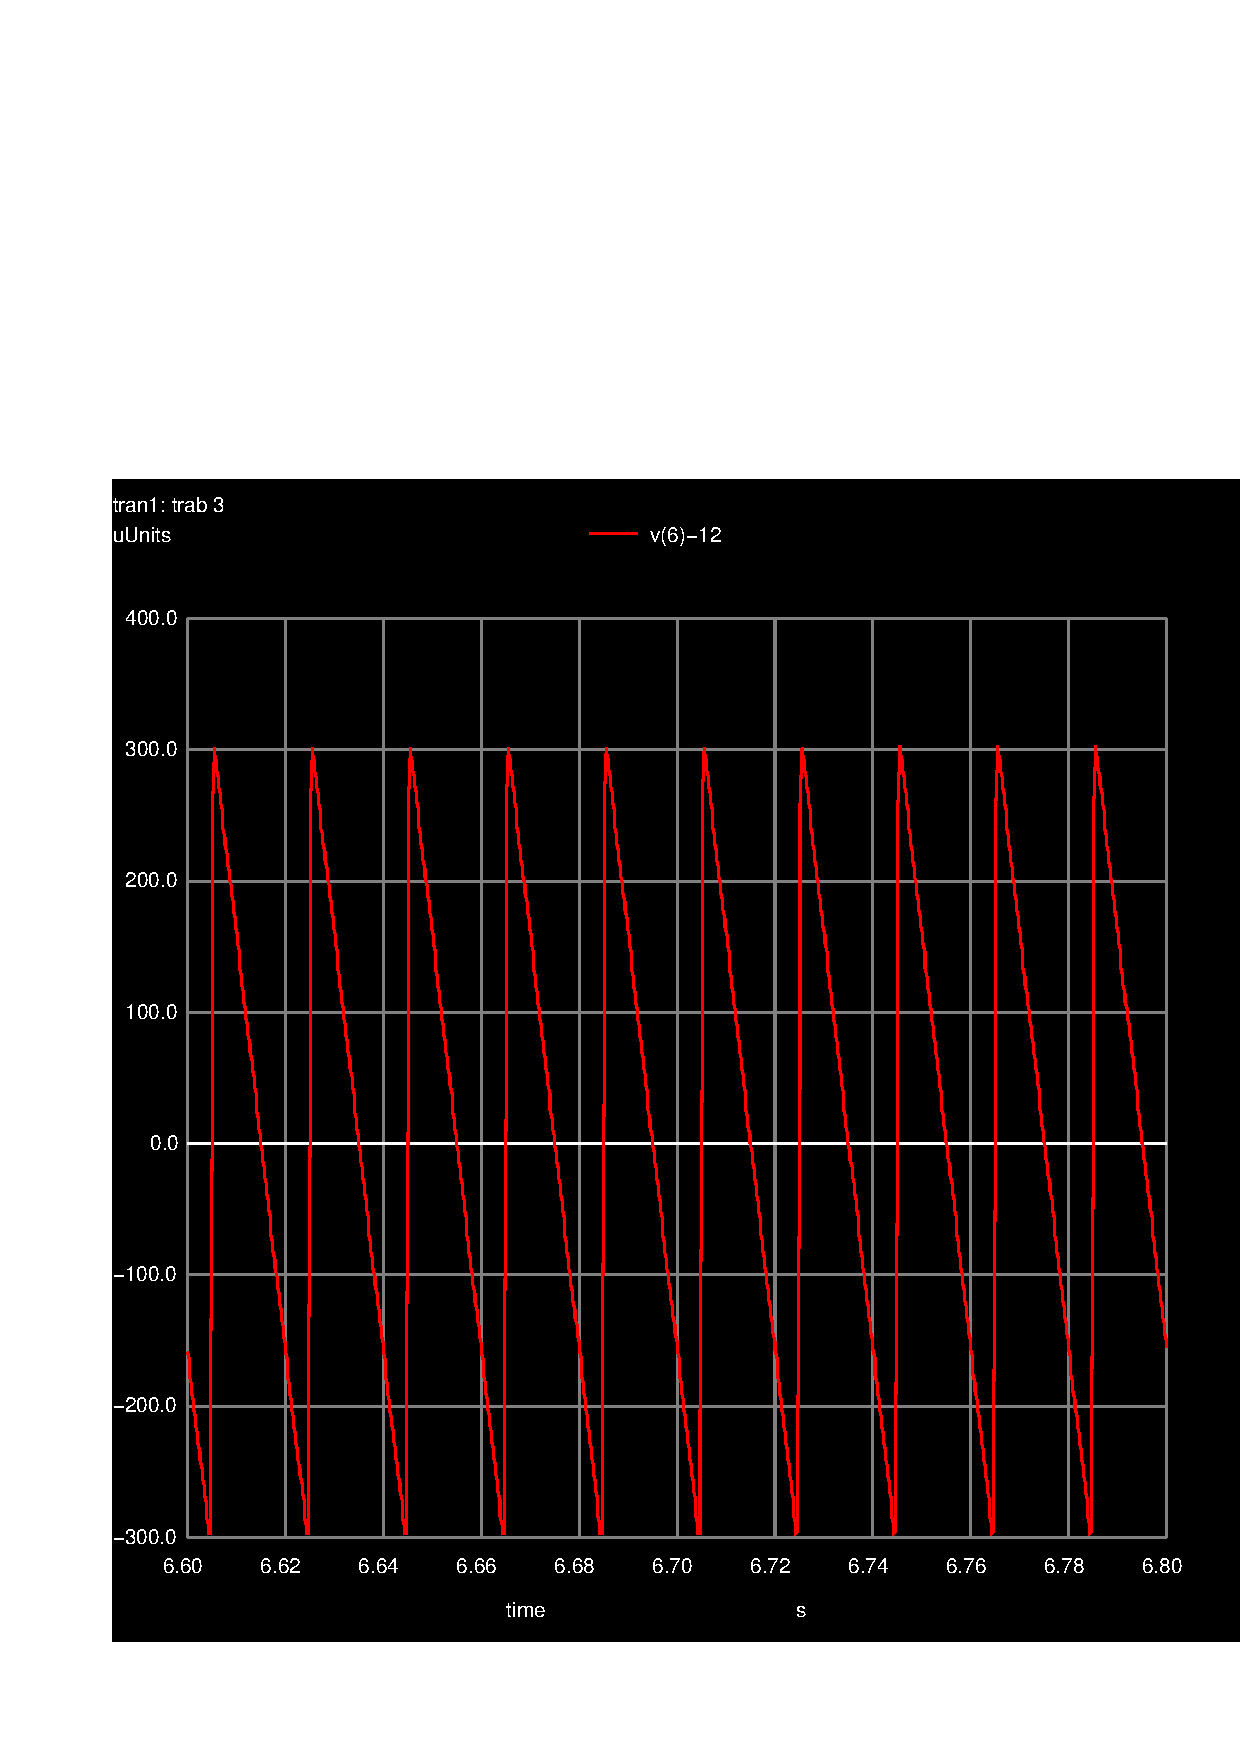
\includegraphics[width = 0.85\linewidth]{sim/deviation.pdf}
    \vspace*{-10mm}
        \caption{\textit{Plot of the difference between the circuit's output voltage and the desired voltage, $V=12V$}}
    \label{fig:dev}
\end{figure}

which, numerically, gives: INSERT HERE

\begin{equation}
    |v_6 - 12| = 
\end{equation}

\section{Theoretical Analysis}

The theoretical analysis can be subdivided in 3 parts

\subsection{DC analysis}
For the DC part, we followed a similar thought to the first code the teacher had which is: the capacitors block the current going through it! However, we chose to calculate the currents in such a way as to not divide the circuit in the same way the teacher's code did. Thus, if we define $I_{xi}$, where $x$ can be $c, e, b$ and $i$ $1, 2$, as being the currents going in the collector, emitter and base, for each of the transistors, respectively, and $I_{R1}$ and $I_{R2}$ to be the currents going through the resistors $R_1$ and $R_2$, we can then retrieve all the important information from the circuit using the matrix in \eqref{eq:dcmatrix}.

\begin{equation}
\scalemath{0.7}{
    \begin{bmatrix}
     -\beta_1 & 1 & 0 & 0 & 0 & 0 & 0 & 0\\
     0 & 0 & 0 & -\beta_2 & 1 & 0 & 0 & 0\\
     1 & 0 & 0 & 0 & 0 & 0 & -1 & 1\\
     1 & 1 & -1 & 0 & 0 & 0 & 0 & 0\\
     0 & 0 & 0 & 1 & 1 & -1 & 0 & 0\\
     0 & 0 & 0 & 0 & 0 & 0 & R_2 & R_1\\
     0 & R_c & R_e & R_c & 0 & 0 & 0 & 0\\
     0 & 0 & 0 & 0 & 0 & R_{out} & 0 & 0
    \end{bmatrix} 
    \begin{bmatrix}
        I_{b1}\\
        I_{c1}\\
        I_{e1}\\
        I_{b2}\\
        I_{c2}\\
        I_{e2}\\
        I_{R1}\\
        I_{R2}
    \end{bmatrix}
    =
    \begin{bmatrix}
        0\\
        0\\
        0\\
        0\\
        0\\
        -V_{cc}\\
        V_{cc}-V_{beon}\\
        V_{cc}-V_{beon}
    \end{bmatrix}}
\label{eq:dcmatrix}
\end{equation}
 
This then allows to for the calculation of $g_m$, $r_\pi$ and $r_o$ using the equations below.
\begin{gather}
    g_m = I_c/V_T\\
    r_\pi = \beta/g_m\\
    r_o = V_{AFN}/I_c
\end{gather}
Where each parameter is calculated for each transistor, according to the respective $\beta$ and $I_c$.
This also allows for the calculation of the output and input impedances for each stage,
\begin{gather}
    Z_{I1} = \frac{1}{\frac{1}{R_B}+\frac{r_{o1}+R_c+R_e}{(r_{o1}+R_c+R_e)(R_{\pi 1}+R_e)+g_{m1}R_er_{o1}r_{\pi 1} - R_e^2}} \\
    Z_{O1} = \frac{1}{\frac{1}{r_{o1}}+\frac{1}{R_c}}\\
    Z_{I2} = \frac{g_{m2} + g_{\pi 2} + g_{o2} + g_{e2}}{g_{\pi 2}}(g_{\pi 2} + g_{o2} + g_{e2})\\
    Z_{O2} = \frac{1}{g_{m2} + g_{\pi 2} + g_{o2} + g_{e2}}
\end{gather}

Through Octave, we get Tab.  \ref{tab:my_label}.

\begin{table}[H]
    \centering
    \begin{tabular}{c|c}
    \hline
    $Z_{I1} (\Omega)$ & $Z_{O1}(\Omega)$\\
    \hline
    $8006.605727$ & $876.533673$
    \hline
    $Z_{I2} (\Omega)$ & $Z_{O2}(\Omega)$\\
    \hline
    $6975.564760$ & $0.220603$
    \hline
    \end{tabular}
    \caption{Input and output impedances for the gain and output stages.}
    \label{tab:my_label}
\end{table}

We can also calculate immediately the total impedance through \eqref{eq:totimpd} and the value is presented in Tab. \ref{tab:totimpd}.

\begin{equation}
    Z_O = \frac{1}{g_{o2} + \frac{g_{m2}}{g_{\pi 2}}g_B + g_{e2} + g_B}
    \label{eq:totimpd}
\end{equation}

\begin{table}[H]
    \centering
    \begin{tabular}{c|c}
    \hline
    $Z_{O} (\Omega)$ & 
    $9.152525$\\
    \hline
    \end{tabular}
    \caption{Total output of the stages.}
    \label{tab:totimpd}
\end{table}

\subsection{Incremental analysis}
As for the incremental analysis, the DC voltage source $V_{cc}$ is shut down and so the nodes 0 (ground) and 6 are merged together and the transistors are approximated by the model that includes 2 capacitors, 2 resistors and a dependent voltage source (model needed in order to capture the higher cutoff frequency in the theoretical analysis). The circuit analysed in this part is presented bellow.

\begin{figure}[H]
    \centering
    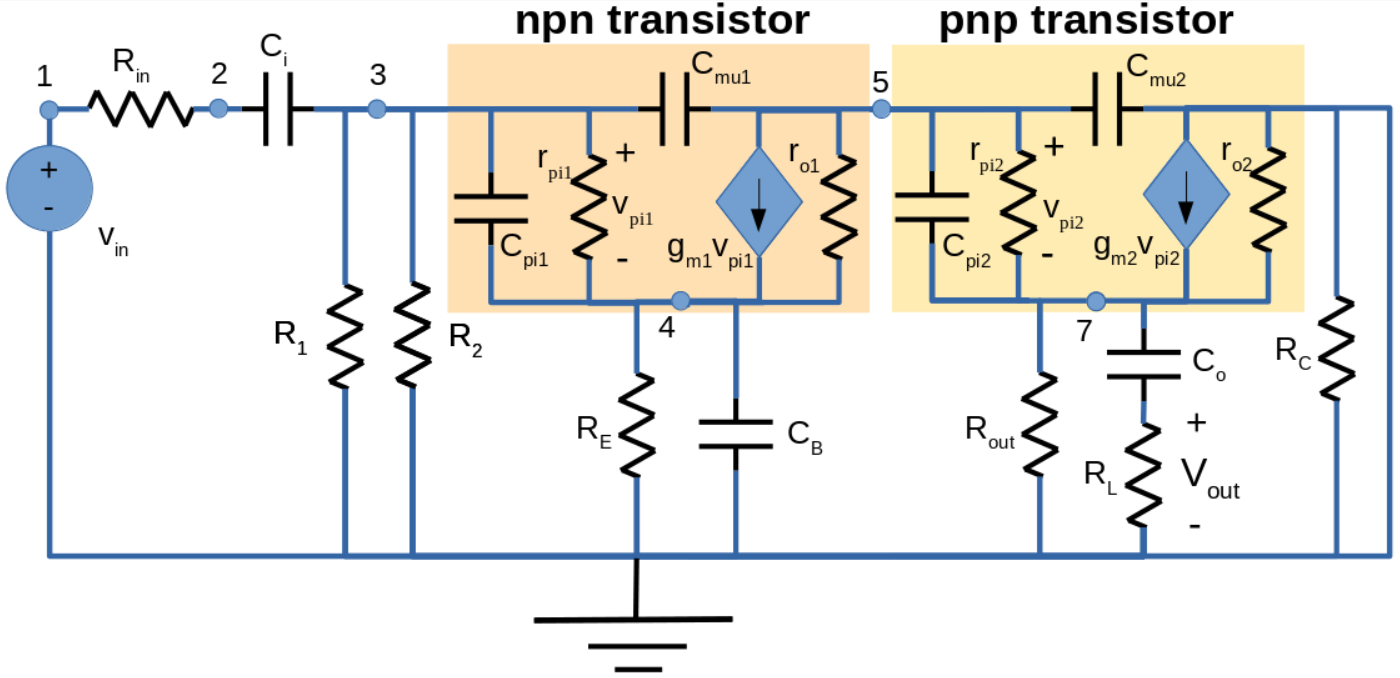
\includegraphics[width = 0.85\linewidth]{ac_analisys_circuit.png}
            \caption{\textit{Circuit in the incremental analysis. There is no node 6 because it was merged with ground.}}
    \label{fig:incrementalscheme}
\end{figure}

Then the nodal analysis method is applied in order to obtain in the end the output of each stage, which is $V_5$ and $V_{out}$. In order to simplify this method, $R_{in}$ and $C_i$ are merged into $Z_{in}$, disappearing node 2. Same process is applied in $R_E$ and $C_B$ that are in parallel, creating $Z_{DE}$. It is also defined $V_{0}=0$, because it's ground and $V_{1}-V_{0}=V_{in}$, which leaves only nodes 3, 4, 5, 7 and 8 for analysis.


\begin{equation}
    \begin{cases}
        \frac{V_3-V_{in}}{Z_{in}}+\frac{V_3-V_0}{R2}+\frac{V_3-V_0}{R1}+\frac{V_3-V_4}{R_{\pi1}}+(V_3-V_4)i \omega C_{\pi1}+(V_3-V_5)i \omega C_{\mu1}=0 \hspace{5mm}\text{(node 3)}\\
        \frac{V_4-V_3}{R_{\pi1}}+\frac{V_4-V_0}{Z_{DE}}+\frac{V_4-V_5}{r_{o1}}-g_{m1}(V_3-V_4)=0 \hspace{5mm}\text{(node 4)}\\
        g_{m2}(V_3-V4)+\frac{V_5-V_4}{r_{o1}}+(V_5-V_3)i \omega C_{\mu1}+\frac{V_5-V_0}{r_{C}}+(V_5-V_0)i \omega C_{\mu2}+(V_5-V_7)i \omega C_{\pi2}+\frac{V_5-V_7}{r_{\pi2}}  = 0 \hspace{15px}\text{(node 5)}\\
        (V_7-V_5)i \omega C_{\pi2}+\frac{V_7-V_5}{r_{\pi2}}+\frac{V_7-V_0}{r_{out}}+(V_7-V_8)i \omega C_o -g_{m2}(V_5-V_7)+\frac{V_7-V_0}{r_{o2}}  = 0 \hspace{15px}\text{(node 7)}\\
        (V_8-V_7)i \omega C_o+\frac{V_8-V_0}{r_{L}}  = 0 \hspace{15px}\text{(node 8)}\\
    \end{cases}
\end{equation}

Which is equivalent to the matrix form that is to be solved in Octave.

\begin{equation}
\scalemath{0.7}{
    \begin{bmatrix}
     G_{in}+G_2+G_1+G_{\pi1}+i\omega C_{\mu1} &  -G_{\pi1}      &  -i\omega C_{\mu1} &    0  &     0      \\
     -G_{\pi1}-g_{m1} & G_{\pi1}+G_{DE}+G_{o1}+g_{m1} & -G_{o1}  & 0   &  0      \\
     g_{m1}-i\omega C_{\mu1}   & g_{m1}-G_{o1}    & G_{o1}+G_C+G_{\pi2}+i\omega C_{\mu1}+i\omega C_{\mu2}  &  -G_{\pi2}-i\omega C_{\mu2}   &   0       \\
     0   & 0        & -G_{\pi2}-g_{m2}   & G_{\pi2}+G_{o2}+G_{out}+g_{m2}+i\omega C_{o} & -i\omega C_{o}      \\
     0   &  0      &  0 &  -i\omega C_{o}  &   i\omega C_{o}+G_L\\
    \end{bmatrix} 
    \begin{bmatrix}
        V_3\\
       V_4\\
        V_5\\
        V_7\\
        V_8\\
    \end{bmatrix}
    =
    \begin{bmatrix}
        V_{in}G_{in}\\
        0\\
        0\\
        0\\
        0
    \end{bmatrix}}
\label{matrix_octave_incremental}
\end{equation}
\section{Side by Side Comparison}

In this section, one can check the responses from the two simulations.

\begin{table}[H]
    \begin{minipage}{.5\textwidth}
    \centering
    \vspace{3mm}
    \begin{table}[H]
    \centering
    \begin{tabular}{|c|c|}
    	\hline
        Variable & Unit [Hz, dB, -, -]\\ 
        \hline
        Central Frequency & 1053.65\\
        \hline
        Gaindb & 40.1602\\
        \hline
        Merit & 8.53488e-6\\
        \hline
        Clean Merit & 3.29139e-5\\
        \hline
    \end{tabular}
	\end{table}
    \caption{Theoretical analysis.}
    \end{minipage}
    \begin{minipage}{.5\textwidth}
        \begin{table}[H]
    \centering
    \begin{tabular}{|c|c|}
    	\hline
    	Variable & Unit [Hz, MU, dB, -, -]\\ 
    	\hline
         \input{../sim/values_tab}
    \end{tabular}
	\end{table}
	\caption{Simulation analysis.} 
    \end{minipage}
\end{table}


\begin{table}[H]
    \begin{minipage}{.5\textwidth}
    \centering
    \vspace{3mm}
    \begin{table}[H]
    \centering
    \begin{tabular}{|c|c|}
    	\hline
        Impedance &  [VA]\\ 
        \hline
        $Z_{in}$ & 1000.00 + i(-686.595)\\ \hline
        $|Z_{in}|$ & 1213.02\\ \hline
        $Z_{out}$ & 669.582 + i(-110.422)\\ \hline
        $|Z_{out}|$ & 818.280\\ \hline
    \end{tabular}
	\end{table}
    \caption{Theoretical analysis.}
    \end{minipage}
    \begin{minipage}{.5\textwidth}
     \begin{table}[H]
    \centering 
    \begin{tabular}{|c|c|}
    	\hline
    	Impedance & [VA]\\ 
    	\hline
         Zi & 1385.89 + (-36.7344)j $\Omega$\\ \hline
|Zi| & 1386.38 $\Omega$\\ \hline

         Zo & 14.0507 + (0.625162)j $\Omega$\\ \hline
|Zo| & 14.0646 $\Omega$\\ \hline

    \end{tabular}
	\end{table}
	\caption{Simulation analysis.} 
    \end{minipage}
\end{table}

\begin{table}[H]
    \begin{minipage}{.5\textwidth}
    \centering
    \begin{figure}[H]
    \centering
    \includegraphics[width = \linewidth]{../mat/gain_banda.png}
	\end{figure}
    \caption{Theoretical analysis.}
    \end{minipage}
    \begin{minipage}{.5\textwidth}
	\begin{figure}[H]
    \centering
    \includegraphics[width=\linewidth]{../sim/voutfreq.pdf}
	\end{figure}
	\caption{Simulation analysis.} 
    \end{minipage}
\end{table}


\section{Presential Laboratory}
In this laboratory, for the first time in this semester, we were able to attend to a laboratory in person which allowed us to better understand how to design and implement the band-pass filter that we were proposed to in this laboratory assignment using an OP-AMP and undoubtedly to better understand how this circuit works. So, and in order to compare with the circuits built and the components used on the remote work, we took some photos of the circuit and took notes of some relevant values.\\

First, on when it comes to the circuit, it is very similar to the one used on the remote work analysis, but with some differences due to limitations of the components available on the laboratory. Thus, for this circuit we only used $220nF$ capacitors and to distinguish the part that corresponded to the high-pass filter and to the low-pass filter we used different types of resistors (higher values to the high-pass filter - we used a $1k\Omega$ resistor $R_1$ - and lower values to the low-pass filter - where we used two $1k\Omega$ resistors in parallel to achieve a $500\Omega$ resistor $R_2$). For the resistors $R_3$ and $R_4$ we used $1k\Omega$ and $2k\Omega$, respectively. A scheme of the circuit can be seen in Fig. \ref{fig:esquemalab} and a photo of it in Fig. \ref{fig:fotolab}

\begin{figure}[H]
    \centering
    \includegraphics[width=\linewidth]{presentialscheme.pdf}
    \caption{Scheme of the circuit used on the laboratory.}
    \label{fig:esquemalab}
\end{figure}

\begin{figure}[H]
    \centering
    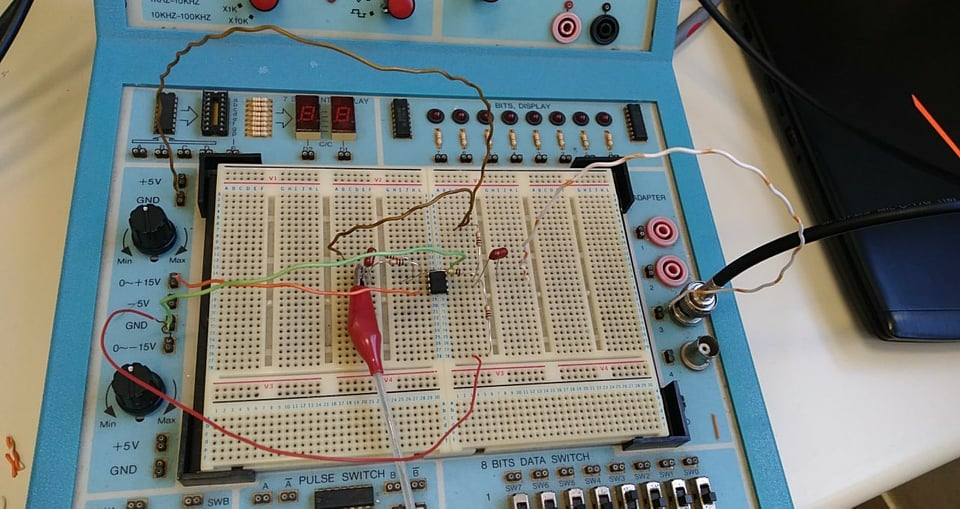
\includegraphics[width=\linewidth]{fotolab.jpg}
    \caption{Photo of the used circuit on the laboratory.}
    \label{fig:fotolab}
\end{figure}

The goals for this work were very similar to the ones for the remote work: amplify an input signal and get a central frequency of $1kHz$ for it. So, in order to better understand how far (or not) we remained from the objectives that were set, we registered the values obtained for the lower and the higher cutoff frequencies (that are, of course, affected with some uncertainty that can't be exactly quantified). The registered values are presented on equation \eqref{values}

\begin{equation}
    f_L = 711Hz \hspace{40px} f_H = 1330Hz
    \label{values}
\end{equation}

Once again, and similarly to what we have done for the remote work, one can find the central frequency of the signal by calculating the geometric mean of the lower and higher cutoff frequencies (definition which results directly from the definition of the transfer function for this circuit). So, we obtain the following value for the central frequency of the signal which is presented on equation \eqref{centraldoff}

\begin{equation}
    central frequency = \sqrt{f_L f_H} \approx 972.435Hz
    \label{centraldoff}
\end{equation}

The value obtained is pretty satisfactory, being sufficiently close enough to the desired value of $1kHz$. To better quantify how far we ended to the desired value, one can calculate the experimental error, which gives an (excellent) value of $\epsilon (\%) = 2.76\%$.
\section{Conclusion}
In this laboratory assignment, as presented above, we were proposed to build and study the behaviour of an AC/DC converter. To build it, one used an envelope detector circuit (composed by a full-wave rectifier which turns the AC input into a DC output and a capacitor which smooths the oscillating current) and a voltage regulator circuit (that uses a resistor and multiple diodes which limit the output voltage to the desired value - 12V).\\

To evaluate how good the built converter was, we recurred the merit score presented in \eqref{score}. The results obtained in the simulation analysis (section 2) were very satisfactory except the stabilization time of the circuit, but that wasn't taken into account in the score obtained for the circuit although we had in mind that the circuit shouldn't have a very long stabilization time. The results given by the simulation analysis show an output signal with an average value displaced $\sim 10^{-7}$V from the desired value of 12V and with ripples $\sim 10^{-4}$V. The output voltage obtained is thus almost perfectly equal to the desired output voltage for this converter, which shows that the goal of this simulation was successfully achieved.\\

Comparing the simulation and the theoretical results one can notice a significant difference between the plots and the results obtained with both as anticipated on section 2. In fact, this phenomenon can be justified by the multiple approximations made in the theoretical analysis, namely on the diode model used. In the analysis made using \textit{Octave}, one used the diode models presented in class which neglect the non-linear behaviour of these components which ends up introducing discrepancies between the analysis methods used.\\

However, it is also important to notice that the results obtained on the theoretical analysis were affected of very small ripples, not however as small as in the simulation. To get a better approximation of the merit obtained in the simulation part, we proposed a corrected merit as well, which assumes that the average of the output voltage is exactly $12V$.\\

Therefore, and having explained the differences registered between the theoretical and the simulation analysis, it can be stated that the goals for this laboratory assignment were successfully achieved.
\begin{thebibliography}{9}
\bibitem{ngsite} 
Ngspice official website, \textit{http://ngspice.sourceforge.net/}
\end{thebibliography}


\end{document}
